In order to test the robustness of sparse logistic regression (LASSO) for feature selection, we added 5000 extra random features to the dataset and analyzed the classifier's performance. We generated the extra features in accordance to an approximation to Zipf's law. Assuming that we can calculate the frequency of a term by the percentage of times it appears as a non-zero values in the data matrix, the sorted ranking of the frequency of the terms should follow Zipf's law. As this ranking should prove different for terms in documents in the target class compared to terms outside the target class we plotted the rank vs. frequency for the full sorted, target class [yes class], and non-target class [no class] in Figure~\ref{fig:largecompare}b. In Figure~\ref{fig:largecompare}(a) we present the same distributions, all however sorted by the rank of the full matrix. We randomly sample from the generated distribution to determine the frequency of each new randomly generated feature, and randomly select either 1 or 0 for each example with probability equal to the chosen frequency. In this way we generated new features which preserves the characteristics of the original feature space.

\begin{center}
\begin{figure}[!ht]
\centering
\subfloat[Unsorted]{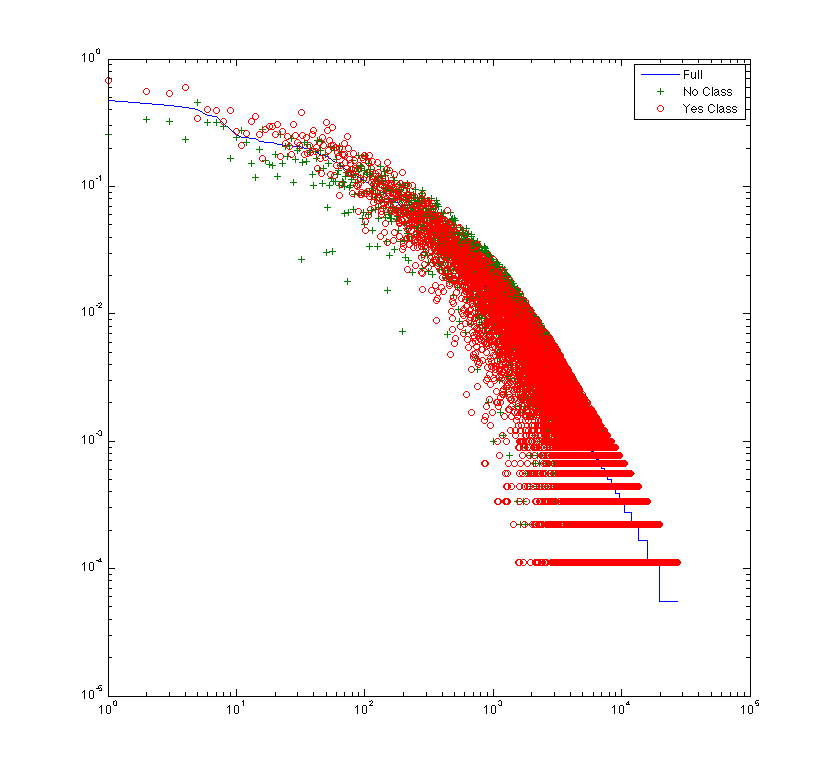
\includegraphics[width=.5\textwidth]{../images/zipfRankedFull.png}}
\subfloat[Sorted]{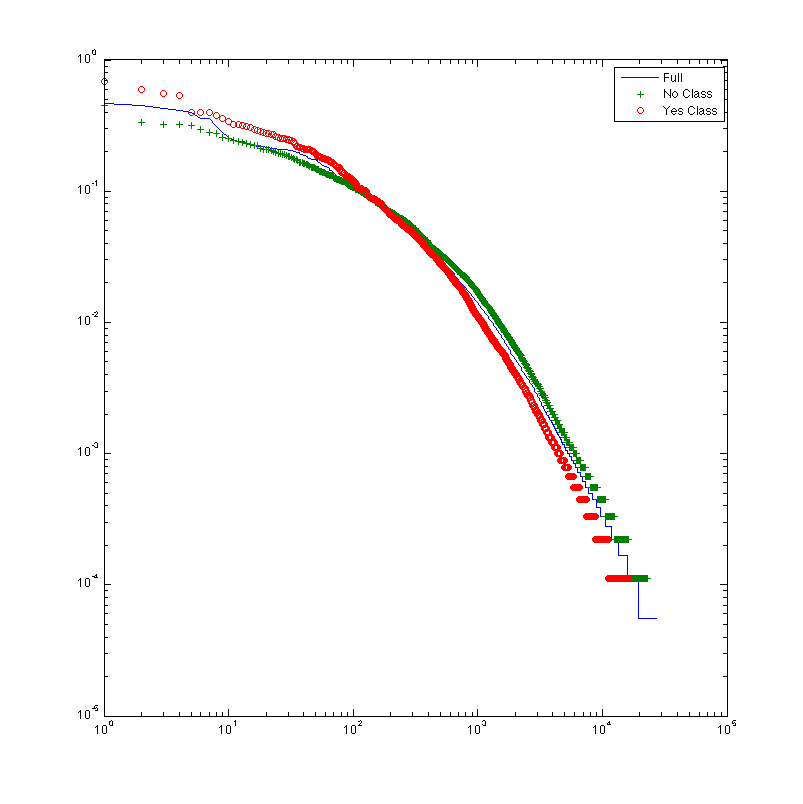
\includegraphics[width=.5\textwidth]{../images/zipfAllSorted.png}}
\caption{Frequency Vs. Rank in full data, target, and other classes}
\label{fig:largecompare}
\end{figure}
\end{center}

\begin{center}
\begin{figure}[!ht]
\centering
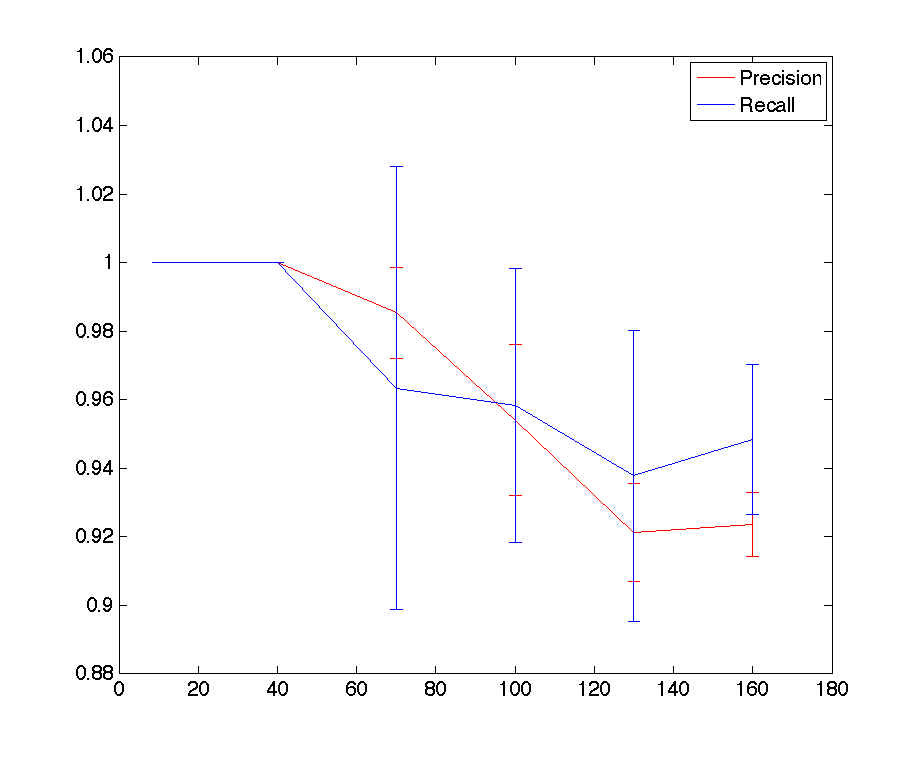
\includegraphics[width=.7\textwidth]{../images/precisionrecallExpansion.png}
\caption{Precision and Recall vs. Number of features selected using LASSO.}
\label{fig:precrecall}
\end{figure}
\end{center}

The experiment for recovering features was performed as follows. We trained a LASSO model on the expanded dataset as well as the original dataset. The best performing $\lambda$ value (weight placed on regularization term) was selected for both using a development set. Classification results on a test set were compared between the model run on the original data and the expanded data. We also calculated the precision and recall of returning the features that LASSO returned on the actual dataset. In other words, we analyzed how well LASSO was able to select the set of salient features it selects when noise features aren't present.  These results can be viewed in Table~\ref{tab:expandedResult}. As can be seen, LASSO is robust for selecting good features even with the addition of random features. The mean accuracy of Expanded and Native are within the error bars of each other. The benefit in terms of classification accuracy of performing LASSO on the native dataset compared to the expanded (calculated as the average of the difference of the accuracy on each run) is none. In terms of being able to recover the original support selected by LASSO, recall is about 94 percent (with a large standard deviation due to one outlier), while precision is considerably lower. When we calculated precision and recall, we computed the best $\lambda$ value for each model by selecting optimal classification peformance on a development set. Though the precision and recall numbers show that LASSO is selecting slightly different sets of features when faced with random noise or not, it seems these non-overlapping features it selects aren't important to the models. The last column shows the number of features we'd have to use until the models selected a different feature. 

In figure~\ref{fig:precrecall}, we vary the size of the feature set selected and plot the precision and recall for each. Here, it can be seen that up to a large number of non-zero weighted features, precision and recall stay at levels larger than 90 percent. The maximum number of features selected by LASSO was about 200.

\begin{table}
\begin{tabular}{lcccccc}
\hline
&Expanded&Native&Benefit&Precision&Recall&Redundant At
\\
\hline
Mean&0.9272&0.9256&-0.0016&0.7570&0.9456&72.5000 \\
STD&0.0099&0.0123&0.0069&0.2913&0.1662&9.6982
\end{tabular}
\caption{Results for expanded dataset feature selection experiment}
\label{tab:expandedResult}
\end{table}